\documentclass[10pt]{beamer}

%presentation settings
\mode<presentation> 
{

  \usetheme{Warsaw}

  \setbeamertemplate{footline}
  {
    \leavevmode%
    \hbox
    {
      \begin{beamercolorbox}[wd=.5\paperwidth,ht=2.5ex,dp=1.125ex,center]{author
      in head/foot}%
      \usebeamerfont{title in head/foot}\insertshortauthor\hspace{.3cm}
      \end{beamercolorbox}%

      \begin{beamercolorbox}[wd=.43\paperwidth,ht=2.5ex,dp=1.125ex,center]{title
      in head/foot}%
      \usebeamerfont{author in head/foot}\hspace{.3cm}\insertshorttitle
      \end{beamercolorbox}%

      \begin{beamercolorbox}[wd=.07\paperwidth,ht=2.5ex,dp=1.125ex,center]{title
      in head/foot}%
      \usebeamerfont{author in
      head/foot}\insertframenumber/\inserttotalframenumber
      \end{beamercolorbox}%
    }
    \vskip0pt%
  }

  \setbeamertemplate{navigation symbols}{} 
  \setbeamertemplate{frametitle}[default][center]
  \setbeamertemplate{caption}[numbered]
  
  \addtobeamertemplate{frametitle}{}{\vspace{-1em}} % decrease
   
  \useinnertheme{rounded}
  \useoutertheme{shadow}
} %end of presentation settings

\usepackage[T2A]{fontenc}
\usepackage{graphicx} 
\usepackage{booktabs} 
\usepackage{mathtools}
\usepackage{sansmathaccent}
\usepackage{mathtext}
\usepackage{amsmath,amsthm, amssymb, latexsym}
\usepackage{fancybox}
\usepackage{color}
\usepackage{xcolor}
\usepackage{verbatim}
\usepackage{ulem}
\usepackage{cancel}
\usepackage{tcolorbox}
\pdfmapfile{+sansmathaccent.map}

\graphicspath{{./Graphs/}}

%Defines
\newcommand*{\boxedcolor}{red}

\newcommand*{\eqlabel}[1]{\label{equation:#1}}
\newcommand*{\typeref}[2]{\ref{#1:#2}}
\newcommand*{\equref}[1]{(\typeref{equation}{#1})}
\newcommand*{\graphref}[1]{Pic.~\typeref{graph}{#1}}
\newcommand*{\fluc}[1]{ #1' }
\newcommand*{\brac}[1]{ \langle #1 \rangle } 
\newcommand*{\ul}[1]{\underline{#1}}
\newcommand*{\ol}[1]{\overline{#1}}
\newcommand*{\vect}[1]{ \arrow{#1} }
\newcommand*{\vectpr}[2]{ \vec{#1} \times \vec{#2} }
\newcommand*{\dotpr}[2]{ \vec{#1} \cdot \vec{#2} }
\newcommand*{\vind}[2]{ {#1}_{#2} }

%----------------------------------------------------------------------------------------
%	TITLE PAGE
%----------------------------------------------------------------------------------------

\title[Linear Algebra In GameDev]{Applications Of Linear Algebra in Game Development.}

\author{Mikhailov V.V.}
\institute[]{}
\date{\today}

\begin{document}

\begin{frame}
\titlepage
\end{frame}

\begin{frame}
\frametitle{Overview} 
\tableofcontents 
\end{frame}

\begin{frame}[t]{Vector, dot and cross product}

\begin{columns}[t,onlytextwidth]
  \column{.45\textwidth}
    \begin{figure}[!htb]
      \begin{minipage}[h]{0.9\linewidth}
      \centering
      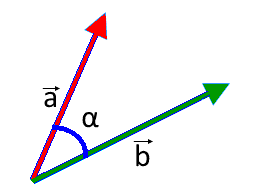
\includegraphics[width = 0.6 \linewidth ]{dot_product.png}
      \caption{\small{For dot product}}
      \label{graph:dot_product}
      \end{minipage}
      \begin{minipage}[h]{1.0\linewidth}
      \centering
      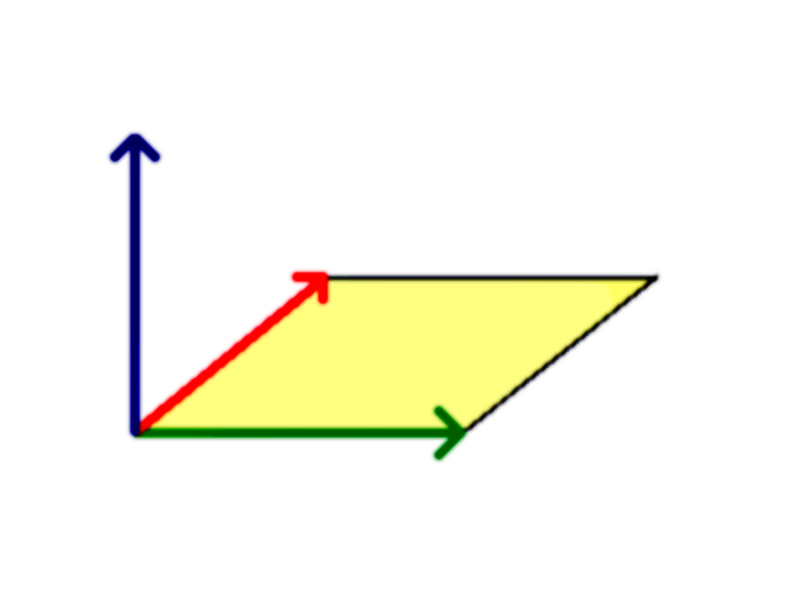
\includegraphics[width = 0.7 \linewidth ]{cross_product.png}
      \caption{\small{For cross product}}
      \label{graph:cross_product}
      \end{minipage}
    \end{figure}
  \column{.55\textwidth}
    \begin{block}{Vector is ...}
     \textit{An element of a \color{red}{vector space}}
    \end{block}
   
    \begin{block}{Basics (assume $\|a\|=\|b\|=1$, $\ \vec{a}, \vec{b} \in R^3 $)}     
      Dot product: $\cos{\alpha} = \dotpr{a}{b} = a^{i} b_i, $ \\
      Cross product:  $|\sin(\alpha)| = \|\vectpr{a}{b}\|$, \\
      where $\vectpr{a}{b} = \begin{vmatrix}
			\vec{i} & \vec{j} & \vec{k} \\
			\vind{a}{x} & \vind{a}{y} & \vind{a}{z} \\
			\vind{b}{x} & \vind{b}{y} & \vind{b}{z} \\
		      \end{vmatrix}
      $ \\
      Wedge product: $\omega = \vec{a} \wedge \vec{b}, \ \omega \in \Lambda^2$
    \end{block}   
    
    \begin{exampleblock}{``Types'' of vectors}
     \begin{itemize}
      \item \textit{Polar}
      \item \textit{Axial (aka pseudovector). }
     \end{itemize}
    \end{exampleblock}   
\end{columns}

\end{frame}

\begin{frame}[t]{Angle between two vectors}
  \begin{columns}[t]
    \column{.45\textwidth}
      \begin{figure}[!htb]
	\centering
	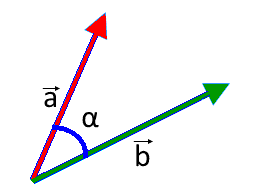
\includegraphics[width = 0.6 \linewidth ]{dot_product.png}
      \end{figure}
    \column{.55\textwidth}
      \begin{tcolorbox}[colback=black!5,colframe=magenta!75!black,title=Problem]
	Find angle $\alpha$ between two vectors $\vec{a}$ and $\vec{b}$
	\tcblower
	\textbf{$\cos{\alpha} = \dotpr{a}{b}$}, but cosine function is an \textit{even} ($\cos{(-\alpha)} = \cos{\alpha}$).
	\color{red}{\textit{sgn} $\alpha$ - ?}
      \end{tcolorbox} 
    \end{columns}
 
      \begin{tcolorbox}[colback=black!5,colframe=yellow!75!black,title=Solution]	
	In general, we need a reference axis $\vec{z}_{ref}$. \\ 
	Let $\vec{z} = \vectpr{a}{b}$. \\ 
	If $\vec{z} \cdot  \vec{z}_{ref} \ge 0$, then $\alpha = \arccos{\dotpr{a}{b}}$, else $\alpha = - \arccos{\dotpr{a}{b}}$. \\
	\textbf{2D case:} Check the sign of $\left| \begin{smallmatrix}
	                                     a_x & a_y \\
	                                     b_x & b_y 
	                                  \end{smallmatrix} 
	                           \right|$

      \end{tcolorbox} 
 
\end{frame}

\begin{frame}[t]{Geometric features}
 \begin{itemize}
  \item $\|\vectpr{a}{b} \| = S_{ABCD}$
  \item $ \frac{1}{2} \|\vectpr{a}{b} \| = S_{ABC}$
  determinant of |a b c|?
  scalar triple product (or mixed product)
  proper and improper rotation
 \end{itemize}

\end{frame}


\end{document}
